%%%%%%%%%%%%%%%%%%%%%%%%%%%%% Define Article %%%%%%%%%%%%%%%%%%%%%%%%%%%%%%%%%%
% sets fontsize to 12
\documentclass[12]{article}
%%%%%%%%%%%%%%%%%%%%%%%%%%%%%%%%%%%%%%%%%%%%%%%%%%%%%%%%%%%%%%%%%%%%%%%%%%%%%%%

%%%%%%%%%%%%%%%%%%%%%%%%%%%%% Using Packages %%%%%%%%%%%%%%%%%%%%%%%%%%%%%%%%%%
\usepackage{geometry}
\usepackage{graphicx}
\usepackage{amssymb}
\usepackage{amsmath}
\usepackage{amsthm}
\usepackage{empheq}
\usepackage{mdframed}
\usepackage{booktabs}
\usepackage{lipsum}
\usepackage{graphicx}
\usepackage{color}
\usepackage{psfrag}
\usepackage{pgfplots}
\usepackage{bm}
\usepackage{changepage}
\usepackage[english]{babel}
\usepackage[colorlinks=true, allcolors=blue]{hyperref}
\usepackage[onehalfspacing]{setspace}
\renewcommand{\familydefault}{\sfdefault}
\usepackage{nicematrix}

%%%%%%%%%%%%%%%%%%%%%%%%%%%%%%%%%%%%%%%%%%%%%%%%%%%%%%%%%%%%%%%%%%%%%%%%%%%%%%%

% extra settings here
% \newcommand\T{\rule{0pt}{2.6ex}}       % Top strut
% \newcommand\B{\rule[-1.2ex]{0pt}{0pt}} % Bottom strut

\newcommand\T{\rule{0pt}{3.5ex}}       % Top strut
\newcommand\I{\rule[-1.25ex]{0pt}{0pt}} % Inner strut
\newcommand\B{\rule[-2.0ex]{0pt}{0pt}} % Bottom strut
\PassOptionsToPackage{table}{xcolor}

%%%%%%%%%%%%%%%%%%%%%%%%%% Page Setting %%%%%%%%%%%%%%%%%%%%%%%%%%%%%%%%%%%%%%%
\geometry{a4paper,top=2.5cm,bottom=2.5cm,left=4cm,right=3cm,marginparwidth=1.75cm}

%%%%%%%%%%%%%%%%%%%%%%%%%% Define some useful colors %%%%%%%%%%%%%%%%%%%%%%%%%%
\definecolor{ocre}{RGB}{243,102,25}
\definecolor{mygray}{RGB}{243,243,244}
\definecolor{deepGreen}{RGB}{26,111,0}
\definecolor{shallowGreen}{RGB}{235,255,255}
\definecolor{deepBlue}{RGB}{61,124,222}
\definecolor{shallowBlue}{RGB}{235,249,255}
%%%%%%%%%%%%%%%%%%%%%%%%%%%%%%%%%%%%%%%%%%%%%%%%%%%%%%%%%%%%%%%%%%%%%%%%%%%%%%%

%%%%%%%%%%%%%%%%%%%%%%%%%% Define an orangebox command %%%%%%%%%%%%%%%%%%%%%%%%
\newcommand\orangebox[1]{\fcolorbox{ocre}{mygray}{\hspace{1em}#1\hspace{1em}}}
%%%%%%%%%%%%%%%%%%%%%%%%%%%%%%%%%%%%%%%%%%%%%%%%%%%%%%%%%%%%%%%%%%%%%%%%%%%%%%%

%%%%%%%%%%%%%%%%%%%%%%%%%%%% English Environments %%%%%%%%%%%%%%%%%%%%%%%%%%%%%
\newtheoremstyle{mytheoremstyle}{3pt}{3pt}{\normalfont}{0cm}{\rmfamily\bfseries}{}{1em}{{\color{black}\thmname{#1}~\thmnumber{#2}}\thmnote{\,--\,#3}}
\newtheoremstyle{myproblemstyle}{3pt}{3pt}{\normalfont}{0cm}{\rmfamily\bfseries}{}{1em}{{\color{black}\thmname{#1}~\thmnumber{#2}}\thmnote{\,--\,#3}}
\theoremstyle{mytheoremstyle}
\newmdtheoremenv[linewidth=1pt,backgroundcolor=shallowGreen,linecolor=deepGreen,leftmargin=0pt,innerleftmargin=20pt,innerrightmargin=20pt,]{theorem}{Theorem}[section]
\theoremstyle{mytheoremstyle}
\newmdtheoremenv[linewidth=1pt,backgroundcolor=shallowBlue,linecolor=deepBlue,leftmargin=0pt,innerleftmargin=20pt,innerrightmargin=20pt,]{definition}{Definition}[section]
\theoremstyle{myproblemstyle}
\newmdtheoremenv[linecolor=black,leftmargin=0pt,innerleftmargin=10pt,innerrightmargin=10pt,]{problem}{Problem}[section]
%%%%%%%%%%%%%%%%%%%%%%%%%%%%%%%%%%%%%%%%%%%%%%%%%%%%%%%%%%%%%%%%%%%%%%%%%%%%%%%

%%%%%%%%%%%%%%%%%%%%%%%%%%%%%%% Plotting Settings %%%%%%%%%%%%%%%%%%%%%%%%%%%%%
\usepgfplotslibrary{colorbrewer}
\pgfplotsset{width=8cm,compat=1.9}
%%%%%%%%%%%%%%%%%%%%%%%%%%%%%%%%%%%%%%%%%%%%%%%%%%%%%%%%%%%%%%%%%%%%%%%%%%%%%%%

%%%%%%%%%%%%%%%%%%%%%%%%%%%%%%% Title & Author %%%%%%%%%%%%%%%%%%%%%%%%%%%%%%%%
\title{Improving on Stab and Gurevychs Argument Component Identification and Classification}
\author{Hugo Meinhof, 815220}
%%%%%%%%%%%%%%%%%%%%%%%%%%%%%%%%%%%%%%%%%%%%%%%%%%%%%%%%%%%%%%%%%%%%%%%%%%%%%%%

\begin{document}
  \maketitle
  \begin{abstract}
  In this article I am presenting new models for classifying and identifying argument components, as defined by Stab and Gurevych\cite{stab-gurevych-2017-parsing}. I propose a new model for running both in one step, as well as models for doing so separately, in a pipeline. I show that my models for the pipeline outperform the baselines, as well as Stab and Gurevychs previous models, on their persuasive essays corpus.
  \end{abstract}
  \section{Introduction\dotfill}
  \subsection{Previous Work: Stab and Gurevych 2017}
  In 2017, Stab and Gurevych\cite{stab-gurevych-2017-parsing} revisited their own work on argumentation mining from 2014. Dissatisfied with the existing corpora at the time, they decided to make their own, which they extended in 2017. On that corpus of persuasive essays, they annotated argument components and their argumentation structures. With these annotations, they trained models to build and test a pipeline. 
  \subsection{Goal of my work}
  For this paper I have attempted to surpass the models for argument component identification and classification, as shown in Figure~\ref{fig:model_tree} \cite{stab-gurevych-2017-parsing}. 
  In general, the identification regards the question of where an argument component, like MajorClaim, will be located, without knowing what type it will be. 
  Then, the classification task is the labeling of what kind of argument component we are dealing with. 
  Stab and Gurevych trained models for each task individually, and my goal was to improve on them. 
  However, I did not work on the argument relation identification, tree generation, or stance recognition. 
  Therefore, I also didn't build a joint model the way they did.
  Nevertheless, I did try to build a model that does the argument component identification and classification in one go, as proposed by Stab and Gurevych.

  ``Another potential issue of the pipeline architecture is that
  wrongly classified major claims will decrease the accuracy of the model because they
  are not integrated in the joint modelling approach. For this reason, it is worthwhile to
  experiment in future work with structured machine learning methods that incorporate
  several tasks in one model (Moens 2013).''\cite{stab-gurevych-2017-parsing}\\
  My attempt at this is discussed later, under the name ``full labels''.

  All of the code I wrote can be found on Github at \href{https://github.com/Theoreticallyhugo/argument_mining_SuG}{``Theoreticallyhugo/argument\_mining\_SuG''}. 
  The models are available on Hugging Face, at \href{https://huggingface.co/Theoreticallyhugo}{``Theoreticallyhugo/longformer-``}, followed by their respective name. 
  \begin{figure}[!h]
    \centering
    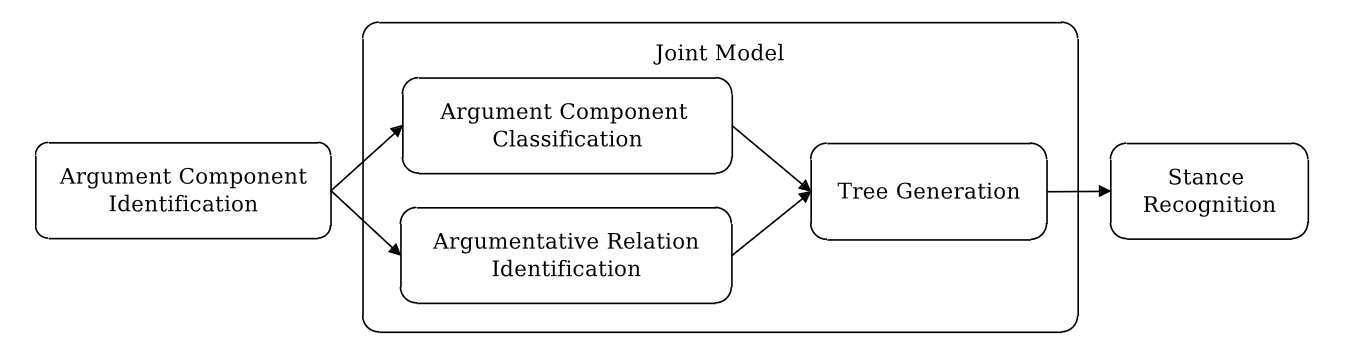
\includegraphics[width=1\linewidth]{../s-g_model_tree.png}
    \caption{Architecture of the argumentation structure parser}
    \label{fig:model_tree}
  \end{figure}
  \subsection{My previous work}
  Prior to this project, I have attempted to achieve what I have achieved now.
  The major difference is switching from bert and similar models to longformer. 
  I assume that this is, because for the project to work, context seems to be one of the most important factors. 
  Bert and its sibling models however tend to be unable to process and therefore ``see'' the texts in their entirety, as they oftentimes are longer than 512 tokens. 
  This means that longformer is the only model to get the entire context all at once.

  \section{Training data\dotfill}
  The foundation of the training data for this project consists of 402 student essays annotated by Stab and Gurevych. 
  For each essay, the dataset includes information on where the core assertion of the text, otherwise known as the MajorClaim, supporting assertments, or the Claims, and the premises, that back up the thesis with statistics and other evidence, are located. 
  The texts used were sourced from essayforum.com and selected randomly. 
  No further information is known about the authors, but it is conceivable that English may not be their first language and they are likely learning it in an educational context.
  Stab and Gurevych subsequently annotated the essays.
  
  The labels they used for annotation are:\\
  \textbf{MajorClaims} build the core opinion. 
  This is what the essay generally argues for or against. 
  They are usually used in the first and last paragraph of the text.\\
  \textbf{Claims} are opinions or statements that support or attack MajorClaims. 
  They usually build the body of the text.\\
  \textbf{Premises} give extra information about Claims, backing them up with examples, statistics, etc.
  They are used as an attempt to make a Claim believable.

  The essays were tokenized and stored where spans are located, what role they have, and which tokens belong to them. 
  In order for models to learn from this, a dataset must be created that processes the data and sorts it comprehensibly to the model. 
  Since all trained models are based on the same data, there is a common dataset for all of them. 
  Many extraction, processing, and matching steps remain the same for all models. 
  Differences basically only exist in the last processing step. 
  This is handled by the different configurations of the dataset. 
  There is a separate configuration for each model, which has the same name as the model. 
  Since the models only differ in how the training data are processed, this also means that a training script can be used for all models, in which only the configuration needs to be adjusted. 
  I also made sure that the configurations have the same names as the models, so that everything runs smoothly, providing a better generalisation of the training script. 
  However, this hasn't always been the case. 
  I started with a separate training script for each model. 
  While this is not as adaptable as a script for all, which can be adjusted via command line arguments, it has the clear advantage that a single model can be trained and tested first, without having to keep others in mind.

  \section{Training\dotfill}
  All training was done using longformer\cite{beltagy2020longformer} and the Hugging Face transformers library. 
  It is a Hugging Face dataset and the code for it, the training, as well as the model weights is public. 
  The corpus, that has been made by Stab and Gurevych \cite{stab-gurevych-2017-parsing}, is publicly available and provided by the University Darmstadt. 
  However, I am not allowed to publish, retransmit, display, redistribute, reproduce or commercially exploit the data in any form, as stated by the license agreement. 
  Therefore the dataset requires acquiring the corpus separately.\\
  The models are evaluated at each epoch for 20 epochs, five times each for the 5-fold cross-validation. 
  All evaluation files are saved in the respective models directory. 
  A separate script collects all evaluation files, calculates the cross-validation and saves the scores to the meta\_data directory for human evaluation. 
  An additional script compiles the macro-f1 scores into the code to build a LaTeX table.\\
  Training has been run on a single Nvidia RTX 4090, as well as an RTX 1080TI separately. This means that the training is optimised for older consumer hardware too.

  \section{The models}
  I have trained and compared multiple models and methods for both identifying and classifying argumentation components. 
  From that process five different models emerged in various stages of simplification and mutual support. 
  All of them are finetuned versions of longformer\cite{beltagy2020longformer}, the long document transformer. 
  \subsection{Full labels} \label{full labels}
  Just like Stab and Gurevych recommended in 2017, I tried to train a model that combined the tasks of argument component identification and classification. For that I used the labels ``B-MajorClaim'', ``I-MajorClaim'', ``B-Claim'', ``I-Claim'',``B-Premise'', ``I-Premise'', and ``O''. 
  The first part of each label carries information for the argument component identification, whilst the second part does so for the classification. 
  Full labels performs worse than Stab and Gurevychs ILP-balanced model\cite{stab-gurevych-2017-parsing}. 
  However this is not an apples to apples comparison, as there is no 5-fold cross-validated evaluation data available for the pipeline, with the ILP model, meaning that it may perform worse than the full labels model. 
  \subsection{Spans} \label{spans}
  Once again, just like Stab and Gurevych in 2017, I came to realise that splitting up the argument component identification and classification could yield overall improvements. 
  The spans model takes care of the first part of the pipeline, the identification. 
  It uses the labels ``B'', ``I'', and ``O''. Reducing the number of labels from seven to three, and limiting the task to identifying the spans, greatly improved the model's performance, compared to full labels.
  \subsection{Simple} \label{simple}
  With the performance increase of the spans model in mind, I created the simple model. It uses the labels ``MajorClaim'', ``Claim'', ``Premise'', ``X\_placeholder\_X'', and ``O''. 
  The ``X\_placeholder\_X'' label however is never annotated in the entire dataset, and hence never used. It is discussed in the section \ref{the placeholder label}.\\
 The idea of this model is the exact same as with the simple model, except this time it's for the classification task instead of identification. The lack of information regarding where spans are, would be made up for in the post processing. There, for each span that has been found by the spans model, the pipeline would check what labels were annotated. The most commonly annotated label within the span would then be applied to the entire span.  
  \begin{verbatim}
``we'', ``should'', ``attach'', ``more'', ``importance'', ``to'', ``cooperation''
``O'', ``Claim'', ``Claim'', ``Premise'', ``Premise'', ``Claim'', ``Claim''
  \end{verbatim}
  \vspace{-3.5ex}
  This synthetic example shows a span without its context. Within it, Claim is the most commonly annotated label, and so the post processing would consider the entire span to be of the type ``Claim''.\\ 
  I did not build a pipeline for the spans model, as it performs worse than sep tok \ref{sep tok}. 
  Therefore all evaluation scores are just from raw comparison to gold, without a pipeline and any pre or postprocessing.
  \subsection{Sep tok full labels} \label{sep tok full labels}
  This model takes advantage of another way in which the spans model can support a model that follows. 
  Not only can the information on where spans are be used during postprocessing, but also before the inference or training. 
  The preprocessing for this model places class and separator tokens in the text data, in order to signal where spans are. 
  They are learned during pretraining and defined in the Hugging Face documentation of longformer as follows:
  \vspace{1ex}
  \begin{adjustwidth}{0.5cm}{0.5cm}
  cls\_token: \verb|<s>|\\
    ``The classifier token which is used when doing sequence classification (classification of the whole sequence instead of per-token classification). It is the first token of the sequence when built with special tokens.'' \cite{LongformerTokenizer} \vspace{1ex}\\
  sep\_token: \verb|</s>|\\
  ``The separator token, which is used when building a sequence from multiple sequences, e.g. two sequences for sequence classification or for a text and a question for question answering. It is also used as the last token of a sequence built with special tokens.'' \cite{LongformerTokenizer}\vspace{-2ex}\\
  \end{adjustwidth}
  So, the model uses the same labels as the full labels model, ``B-MajorClaim'', ``I-MajorClaim'', ``B-Claim'', ``I-Claim'',``B-Premise'', ``I-Premise'', and ``O'', but differentiates itself through the text it is being fed. This means that for this model, input looks like in this synthetic example:
  \begin{verbatim}
``<s>'', ``we'', ``should'', ``attach'', ``more'', ``</s>'', 
``O'', ``B-Claim'', ``I-Claim'', ``I-Claim'', ``I-Claim'', ``O''
  \end{verbatim}
  \vspace{-3.5ex}
  Since injected cls and sep\_token increase the total number of tokens, they are assigned the ``O'' label, in order to keep the labels aligned.
  \subsection{Sep tok} \label{sep tok}
  Both the models simple (\ref{simple}) and sep tok full labels (\ref{sep tok full labels}) showed improvements over the initial full labels model (\ref{full labels}). 
  Therefore, this model was created, taking advantage of both ideas. 
  It uses the labels ``MajorClaim'', ``Claim'', ``Premise'', ``X\_placeholder\_X'', and ``O'', just like simple, and processes texts with inserted separation tokens, like sep tok full labels. 
  It comes to no surprise then, that this model performs better than simple and sep tok full labels.
  \subsection{Pipeline} \label{pipeline}
  The pipeline handles argument component identification and classification individually, and uses the best model for each task. 
  Running the pipeline starts with inference on the input strings, with the spans model. 
  The inference is handled by the Hugging Face pipeline object. 
  Its output is then used to inject class and separation tokens into the input strings. 

  Due to the problems described in \ref{aci-prob}, the following assumptions are made in postprocessing, before injecting tokens: \\
  For any span that begins with ``I'' instead of ``B'', the first ``I'' label is considered the begin. \\
  Any span that is shorter than four tokens is considered an uninterpretable leftover, and hence ignored.  \\
  In order to better understand the model's outputs, and how they are postprocessed, I build a pipeline concerned with spans only. 
  It is called spans\_pipe\_visual and uses colour to indicate where in a text a span is recognised and where it should or should not be recognised.

  The resulting texts are then fed into the sep tok model, once again handled by a Hugging Face pipeline. 
  Its outputs are used in conjunction with the inputs. 
  First, the cls and sep tokens are used to identify the spans within each text. 
  Then, all tokens that lie within each span are found, counted, the most frequent for each identified and then applied to the entire span. 
  If a span is identified, but not labeled, because sep tok labeled all tokens within it as ``O'', it is deleted.

  The resulting information on where spans are and what their label is, is then compiled into the brat standoff format, just like the original data provided by Stab and Gurevych \cite{stab-gurevych-2017-parsing}. This means that the pipeline can take any text and annotate Stab and Gurevychs Argument components, in the same style as their human annotators did with brat.
  \subsection{Problems} \label{problems}
  \subsubsection{Argument component identification} \label{aci-prob}
  Distinguishing between ``B'' and ``I'' labels is supposed to allow proper identification of where spans begin and end. 
  However, there are multiple ambiguous situations, which complicate the process. 

  If, for example, a span starts out with an ``I'' label, it is unclear whether this truly is where the span begins. 
  Possibly this ``I'' label is correct, but should be preceeded by a ``B'' label, but it could also be the case that it isn't correct, and that the ``I'' should be a ``B''. 
  There also are situations where after a span, there is one ``O'', followed by a couple of ``I'' labels. 
  Here, a third possibilty is added, being that this gap should be filled with an ``I'', making it one long span.

  Additionally, there are situations in which an argument component seems to be identified correctly, but classified inconsistently. 
  The ``B'' and ``I'' part of the labels would be fitting perfectly, but for some reason the model annotates Claim five times, then Premise once, only to keep going with Claim. 
  This is accounted for by doing majority voting on spans.

  This leads to the fourth problem, which is that sometimes the spans model may identify a span, without the sep tok model classfifying it. 
  That results in an empty span, which needs to be deleted due to the lack of completeness in its information.
  \vspace{2ex} \\
  \textbf{Problem 1:}
  \vspace{-1.5ex}
  \begin{verbatim}
``we'', ``should'', ``attach'', ``more'', ``importance'', ``to'', ``cooperation''
``O'',  ``I'',      ``I'',      ``I'',    ``I'',          ``I'',  ``I''
  \end{verbatim}
  \vspace{-4ex}
  \textbf{Possible resolutions:}\\
  \textit{``O'' label is begin, span starts one token earlier}
  \vspace{-1.5ex}
  \begin{verbatim}
``we'', ``should'', ``attach'', ``more'', ``importance'', ``to'', ``cooperation''
``B'',  ``I'',      ``I'',      ``I'',    ``I'',          ``I'',  ``I''
  \end{verbatim}
  \vspace{-4ex}
  \textit{``O'' label is correct, and first inside label should be begin instead}
  \vspace{-1.5ex}
  \begin{verbatim}
``we'', ``should'', ``attach'', ``more'', ``importance'', ``to'', ``cooperation''
``O'',  ``B'',      ``I'',      ``I'',    ``I'',          ``I'',  ``I''
  \end{verbatim}
  \vspace{-2ex}
  \textbf{Problem 2:}
  \vspace{-1.5ex}
  \begin{verbatim}
``we'', ``should'', ``attach'', ``more'', ``importance'', ``to'', ``cooperation''
``B'',  ``I'',      ``I'',      ``O'',    ``I'',          ``I'',  ``I''
  \end{verbatim}
  \vspace{-4ex}
  \textbf{Possible resolutions:}\\
  \textit{Skipped label is begin, making two spans, no gap}
  \vspace{-1.5ex}
  \begin{verbatim}
``we'', ``should'', ``attach'', ``more'', ``importance'', ``to'', ``cooperation''
``B'',  ``I'',      ``I'',      ``B'',    ``I'',          ``I'',  ``I''
  \end{verbatim}
  \vspace{-4ex}
  \textit{Skipped label is inside, making one span, no gap}
  \vspace{-1.5ex}
  \begin{verbatim}
``we'', ``should'', ``attach'', ``more'', ``importance'', ``to'', ``cooperation''
``B'',  ``I'',      ``I'',      ``I'',    ``I'',          ``I'',  ``I''
  \end{verbatim}
  \vspace{-4ex}
  \textit{Skipped label is correct and should be followed by begin, making two spans, with gap}
  \vspace{-1.5ex}
  \begin{verbatim}
``we'', ``should'', ``attach'', ``more'', ``importance'', ``to'', ``cooperation''
``B'',  ``I'',      ``I'',      ``O'',    ``B'',          ``I'',  ``I''
  \end{verbatim}
  \vspace{-4ex}
  \textbf{Problem 3:}\\
  \textit{For readability, the labels ``I-Claim'' and ``I-Premise'' have been shortened to ``I-C'' and ``I-P'' respectively.}
  \vspace{-1.5ex}
  \begin{verbatim}
``we'', ``should'', ``attach'', ``more'', ``importance'', ``to'', ``cooperation''
``B-C'', ``I-C'',   ``I-C'',    ``I-C'',  ``I-P'',        ``I-C'', ``I-C''
  \end{verbatim}
  \vspace{-4ex}
  Additionally there is the issue of rogue labels, meaning that there sometimes are one, two, or three inside-label-long spans at seemingly random positions. 
  For now, any span shorter than three is ignored, but considering the second problem, this could delete important parts or even entire spans, because they are split.
  \subsubsection{The ``X\_placeholder\_X'' label} \label{the placeholder label}
  For some reason CUDA kept crashing on the backwards pass, when the training for token classification of longformer ran with an even number of labels. 
  Therefore, the ``X\_placeholder\_X'' label was introduced. 
  It is never annotated and never part of the model's output, but fixes the issue with CUDA. 
  Hence, I don't think that it influences the performance the models achieve.

  \section{Evaluation\dotfill}
  For reproduceability, every training and inference was seeded. 
  Furthermore, all evaluation was 5-fold cross-validated, just like Stab and Gurevych did with their models, on the same data. 
  However all evaluation is done on the raw inference, without any postprocessing.
  These efforts don't guarantee full reproduceability, but do lead to more stable and comparable scores.

  With a Makro-f1 score of 0.77, the full labels model, running both the argument component identification and classification in one go, already performs quite well. 
  Considering that it's a fast and simple single step solution, it certainly has its perks. 
  It also needs to be mentioned, that the model surpasses the majority and heuristic baselines for both argument component identification and classification as presented by Stab and Gurevych.
  From epoch 7 onward, we get to see very little improvements. 
  Epoch 14 is getting the best results, marking the beginning of a mostly flat curve, followed by very little change in either direction. 
  Interestingly, there seems to be no overfitting within the 20 epochs of training.

  For the argument component identification task, Stab and Gurevych were happy to announce that their model's performance came very close to their human annotators. 
  I am equally happy to announce that the spans model has surpassed both their models, as well as human performance (see table \ref{tab:ident_f1}). 
  Since Table 8 and Table C.1 in \cite{stab-gurevych-2017-parsing} report different scores for CRF all features, both are included in Table \ref{tab:ident_f1}.\\
  The model takes only three epochs to perform very well. 
  Considering scores, there isn't really a point in training beyond five epochs, but from epoch 15 onward, the curve is almost flat. 
  Once again there are no signs of overfitting within the 20 Epochs of training. 

  Out of the three models for argument component classification, the simple model performs the worst. 
  Nevertheless, it achieves better scores than the baselines, the full labels model, and comes somewhat close to the performance of Stab and Gurevychs ILP-balanced model. 
  Comparing simple to their standalone model for classification, SVM all features, it surpasses the scores, as well as the baselines.\\
  In epochs six through 14, the model gets very similar scores, only to be improved upon by about 0.01 five epochs later. 
  Therefore, an f1 of 8.811 can be claimed, but 0.799 at epoch six would be more sensible.\\
  Here too, the scores eventually settle, without really worsening again, indicating that there is no overfitting yet.

  The sep tok full labels model is the first to outperform Stab and Gurevychs ILP-balanced, without being the best in the group yet. 
  Its scores fluctuate throughout the epochs, with the most significant improvements having taken place till epoch eleven and eventual stabilising towards epoch 18.

  Sep tok is the best performing model so far, showing better scores than the baselines, other longformer based, and Stab and Gurevychs models (see table \ref{tab:class_f1}). 
  It gains the most performance until about epoch eight, with fluctuation, but eventual improvements until epoch 16. 
  This is also the only model that shows performance dips after that epoch, meaning that there is no flattening of the curve, as observed with the other models.

  ``Our identification model yields good accuracy and an $\alpha_U$ of 0.958 for identifying argument components. 
  Therefore, it is unlikely that identification errors will significantly influence the outcome of the downstream models when applied to persuasive essays.'' \cite{stab-gurevych-2017-parsing}\\
  Following the reasoning of Stab and Gurevych, I am assuming that the pipeline's performance is very close to that of the downstream model, both for my, as well as their models.
  \begin{table}[!h]
    \centering
    \begin{NiceTabular}{c||c|c|c|c|c}
      \CodeBefore
        \rowcolors{2}{gray!25}{white}
      \Body
      \textbf{Makro-f1} & \textbf{full labels} & \textbf{spans} & \textbf{simple} & \textbf{sep tok full labels} & \textbf{sep tok}\\
      \hline
      \hline
      01 & 0.378 & 0.798 & 0.668 & 0.525 & 0.754\T\\
      02 & 0.522 & 0.889 & 0.743 & 0.670 & 0.810\\
      03 & 0.635 & 0.902 & 0.777 & 0.795 & 0.840\\
      04 & 0.730 & 0.908 & 0.788 & 0.816 & 0.854\\
      05 & 0.743 & 0.912 & 0.792 & 0.818 & 0.863\\
      06 & 0.752 & 0.909 & 0.799 & 0.830 & 0.861\\
      07 & 0.757 & 0.911 & 0.796 & 0.829 & 0.867\\
      08 & 0.759 & 0.911 & 0.798 & 0.833 & 0.870\\
      09 & 0.759 & 0.912 & 0.796 & 0.841 & 0.868\\
      10 & 0.763 & 0.914 & 0.801 & 0.841 & 0.871\\
      11 & 0.765 & 0.911 & 0.800 & 0.845 & 0.872\\
      12 & 0.766 & 0.913 & 0.800 & 0.841 & 0.866\\
      13 & 0.768 & 0.912 & 0.803 & 0.839 & 0.870\\
      14 & \textbf{0.770} & 0.913 & 0.800 & 0.842 & 0.873\\
      15 & 0.767 & \textbf{0.915} & 0.806 & 0.845 & 0.874\\
      16 & 0.770 & 0.914 & 0.807 & 0.844 & \textbf{0.876}\\
      17 & 0.771 & 0.914 & 0.809 & 0.845 & 0.874\\
      18 & 0.770 & 0.914 & 0.809 & \textbf{0.846} & 0.871\\
      19 & 0.771 & 0.915 & \textbf{0.811} & 0.846 & 0.875\\
      20 & 0.770 & 0.915 & 0.810 & 0.847 & 0.874\\
    \end{NiceTabular}
    \vfill
    \caption{5-fold cross-validation of the macro-f1}
    \label{tab:epoch_f1}
  \end{table}


% \begin{table}[!h]
%   \centering
%   \begin{NiceTabular}{c||c|c|c|c|c}
%     \CodeBefore
%       \rowcolors{2}{gray!25}{white}
%     \Body
%     \textbf{Makro-f1} & \textbf{full labels} & \textbf{spans} & \textbf{simple} & \textbf{sep tok full labels} & \textbf{sep tok}\\
%     \hline
%     \hline
%     01 & 0.493 & 0.872 & 0.710 & 0.627 & 0.790\T\\
%     02 & 0.683 & 0.907 & 0.776 & 0.778 & 0.836\\
%     03 & 0.745 & 0.908 & 0.793 & 0.814 & 0.864\\
%     04 & 0.755 & 0.913 & 0.797 & 0.829 & 0.860\\
%     05 & 0.766 & 0.916 & 0.795 & 0.834 & 0.866\\
%     06 & 0.767 & 0.916 & 0.797 & 0.828 & 0.860\\
%     07 & 0.765 & 0.917 & 0.802 & 0.836 & 0.872\\
%     08 & 0.763 & 0.916 & 0.802 & 0.846 & 0.873\\
%     09 & 0.769 & 0.916 & 0.806 & 0.837 & 0.867\\
%     10 & 0.765 & 0.913 & 0.804 & 0.841 & 0.875\\
%     11 & 0.763 & 0.915 & 0.804 & 0.840 & 0.868\\
%     12 & 0.771 & 0.914 & 0.809 & 0.844 & 0.877\\
%     13 & 0.774 & 0.918 & 0.805 & 0.850 & 0.875\\
%     14 & 0.770 & 0.916 & 0.803 & 0.847 & 0.875\\
%     15 & 0.764 & 0.917 & 0.801 & 0.847 & 0.873\\
%     16 & 0.769 & 0.919 & 0.809 & 0.849 & 0.879\\
%     17 & 0.771 & 0.916 & 0.807 & 0.852 & 0.876\\
%     18 & 0.775 & 0.916 & 0.806 & 0.858 & 0.878\\
%     19 & 0.776 & 0.917 & 0.803 & 0.856 & 0.880\\
%     20 & 0.773 & 0.918 & 0.811 & 0.857 & 0.879\\
%     21 & 0.771 & 0.919 & 0.806 & 0.853 & 0.876\\
%     22 & 0.771 & 0.918 & 0.811 & 0.859 & 0.877\\
%     23 & 0.773 & 0.918 & 0.809 & 0.851 & 0.879\\
%     24 & 0.777 & 0.919 & 0.809 & 0.859 & 0.881\\
%     25 & 0.773 & 0.919 & 0.807 & 0.859 & 0.878\\
%     26 & 0.774 & 0.920 & 0.807 & 0.858 & 0.883\\
%     27 & 0.775 & 0.917 & 0.809 & 0.857 & 0.880\\
%     28 & 0.775 & 0.918 & 0.810 & 0.853 & 0.881\\
%     29 & 0.777 & 0.921 & 0.814 & 0.854 & 0.879\\
%     30 & 0.775 & 0.919 & 0.808 & 0.856 & 0.879\\
%     31 & 0.777 & 0.918 & 0.808 & 0.854 & 0.883\\
%     32 & 0.778 & 0.916 & 0.806 & 0.855 & 0.880\\
%     33 & 0.778 & 0.919 & 0.810 & 0.858 & 0.882\\
%     34 & 0.777 & 0.920 & 0.811 & 0.856 & 0.884\\
%     35 & 0.775 & 0.919 & 0.812 & 0.858 & 0.885\\
%     36 & 0.777 & 0.919 & 0.811 & 0.856 & 0.884\\
%     37 & 0.778 & 0.919 & 0.811 & 0.860 & 0.882\\
%     38 & 0.776 & 0.920 & 0.811 & 0.855 & 0.883\\
%     39 & 0.778 & 0.920 & 0.813 & 0.859 & 0.880\\
%     40 & 0.780 & 0.921 & 0.814 & 0.857 & 0.879\\
%     41 & 0.780 & 0.918 & 0.815 & 0.855 & 0.883\\
%     42 & 0.779 & 0.919 & 0.813 & 0.858 & 0.881\\
%     43 & 0.779 & 0.920 & 0.813 & 0.857 & 0.886\\
%     44 & 0.778 & 0.920 & 0.814 & 0.858 & 0.884\\
%     45 & 0.779 & 0.921 & 0.814 & 0.858 & 0.882\\
%     46 & 0.782 & 0.920 & 0.814 & 0.858 & 0.884\\
%     47 & 0.780 & 0.920 & 0.815 & 0.859 & 0.884\\
%     48 & 0.780 & 0.921 & 0.815 & 0.857 & 0.884\\
%     49 & 0.780 & 0.920 & 0.815 & 0.858 & 0.884\\
%     50 & 0.780 & 0.920 & 0.815 & 0.857 & 0.884\\
%   \end{NiceTabular}
%   \vfill
%   \caption{5-fold cross-validation of the macro-f1}
%   \label{tab:epoch_f1}
% \end{table}


  \begin{table}[!h]
    \centering
    \begin{NiceTabular}{c|c}[colortbl-like]
      \large\textbf{Argument Component Identification} &  \large\textbf{Makro-f1}\\ 
      \hline
      \hline
      \textbf{Stab und Gurevytch}& \T \I \\
      \rowcolor{gray!25}
      Human upper bound & 0.886\\
      Baseline majority & 0.259\\
      \rowcolor{gray!25}
      Baseline heuristic & 0.628\\
      \textbf{CRF all features} & \textbf{0.849 or 0.867}\B\\
      \hline
      \textbf{Meinhof} & \T \I \\
      \rowcolor{gray!25}
      \textbf{spans} & \textbf{0.915}\\ 
    \end{NiceTabular}
    \caption{Argument Component Identification (5-fold cross-validation as in Table C.1 of \cite{stab-gurevych-2017-parsing})}
    \label{tab:ident_f1}
  \end{table}

  \begin{table}[!h]
    \centering
    \begin{NiceTabular}{c|c}[colortbl-like]
      \large\textbf{Argument Component Classification} &  \large\textbf{Makro-f1}\\
      \hline
      \hline
      \textbf{Stab und Gurevych} & \T \I \\
      \rowcolor{gray!25}
      Baseline majority & 0.257\\
      Baseline heuristic & 0.724\\
      \rowcolor{gray!25}
      \textbf{SVM all features} & \textbf{0.773}\\
      \textbf{ILP-balanced} & \textbf{0.823}\\
      \rowcolor{gray!25}
      \textit{ILP and CRF pipeline} & no-eval \B \\
      \hline
      \textbf{Meinhof} & \T \I \\
      \rowcolor{gray!25}
      full\_labels & 0.770\\
      simple & 0.811\\
      \rowcolor{gray!25}
      sep\_tok\_full\_labels & 0.846\\
      \textbf{sep\_tok} & \textbf{0.876}\\
      \rowcolor{gray!25}
      \textit{full\_pipe} & \textit{TO-DO}\\

    \end{NiceTabular}
    \caption{Argument Component Classification (5-fold cross-validation as in Table C.2 of \cite{stab-gurevych-2017-parsing})}
    \label{tab:class_f1}
  \end{table}

  \newpage

  \bibliographystyle{alpha}
  \bibliography{../argmin_meinhof_03_2024}
\end{document}
